\subsection{Teori}

\subsubsection{Rotationsmatricer}
Hvis vi vil roterer et punkt eller en vektor omkring nul-punktet i et koordinatsystem kan vi bruge en rotationsmatrix\cite{rotationsmatricer}.
En rotationsmatrix er en matrix der, hvis ganget sammen med en anden matrix, roterer en vektor eller et punkt i et koordinatsystem.
\begin{align}\label{eu_eqn}
  R_x(\theta) = 
  \begin{bmatrix}
    1 & 0 & 0\\ 
    0 & cos \theta & - sin \theta\\ 
    0 & sin \theta & cos \theta
  \end{bmatrix}\\
    R_y(\theta) = 
  \begin{bmatrix}
    cos \theta  & 0 & sin \theta\\ 
    0           & 1 & 0\\ 
    -sin \theta & 0 & cos \theta
  \end{bmatrix}\\
    R_z(\theta) = 
  \begin{bmatrix}
    cos \theta & - sin \theta & 0\\ 
    sin \theta & cos \theta & 0\\
    0 & 0 & 1
  \end{bmatrix}
\end{align}
Indsætter vi mængden af radianer vi vil dreje vores vektor og ganger dem sammen, burde vektoren bliver drejet omkring nul-punktet med netop den mængde radianer.
For at sikre at vi har forstået brugen korrekt, vil vi nu forsøge at dreje en vektor i rummet omkring x-aksen ved hjælp af $R_x$. 
Vi har en vektor u:
\begin{equation}
  U=
  \begin{bmatrix}
    0 & 1 & 5
  \end{bmatrix}
\end{equation}
og rotationsvektor \begin{math}R_x\end{math}
\begin{equation}
  R_x(\theta) = 
  \begin{bmatrix}
    1 & 0 & 0\\ 
    0 & cos \theta & - sin \theta\\ 
    0 & sin \theta & cos \theta
  \end{bmatrix}
\end{equation}
Vi tager prik-produktet af dem, og indsætter 1 Radian i $R_x$:
\begin{align}
  0*0+1*0+5*0&=0\\
  0*0+1*cos(1)+5*sin(1)&=4.75\\
  0*0+1*(-sin(1))+5*cos(1)&=1.86
\end{align}
Og kalder det for vektor V og indsætter både U og V i Geogebra og får den til at udregne vinklen mellem dem:
\begin{figure}[H]
  \center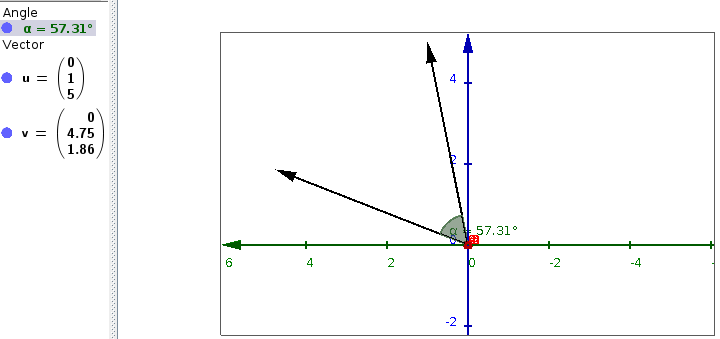
\includegraphics[width=12cm]{rotationsmatrix_eksempel.png}
  \center\caption{Eksempel på en rotationsmatrix}
  \label{fig:rotationsmatrix_eksempel}
\end{figure}
Geogebra udregner vinkler i grader, så vi omregner grader til radianer ved hjælp af ligningen:
\begin{equation}
  R=d/2*\pi/360=57,31/2*\pi/360\approx1
\end{equation}
Dette viser os at vektor $U$ blev drejet 1 radian, som forventet.

\subsubsection{Fra 3D-model til billede}
I dette afsnit er det vist, hvordan der kan udledes en model, der beskriver en billeddannelsen af objekter i rummet, også kaldt rendering. Dette er essentielt da billeddannelsen danner grundlag for, hvordan 3D-modellen for en lampe omdannes til et billede, der kan vises for kunderne på e-butikken. Til sidst i afsnittet udledes en model for, hvordan belysningen fra en lampe kan simuleres og visualiseres vha. raytracing. 

\paragraph{Perspektiv projektion}
For at udlede en model for billeddannelsen, tages der udgangspunkt i en perspektiv projektion. Perspektiv projektion er en måde at danne et billede af 3D-objekter ved at projektere objekterne hen på et plan mod et kameraes position\cite{fig:perspective_projection}. Princippet bag perspektiv projektion er vist på figur \ref{fig:perspektiv_projektion}.

\begin{figure}[H]
  \label{fig:perspektiv_projektion}
  \centering
  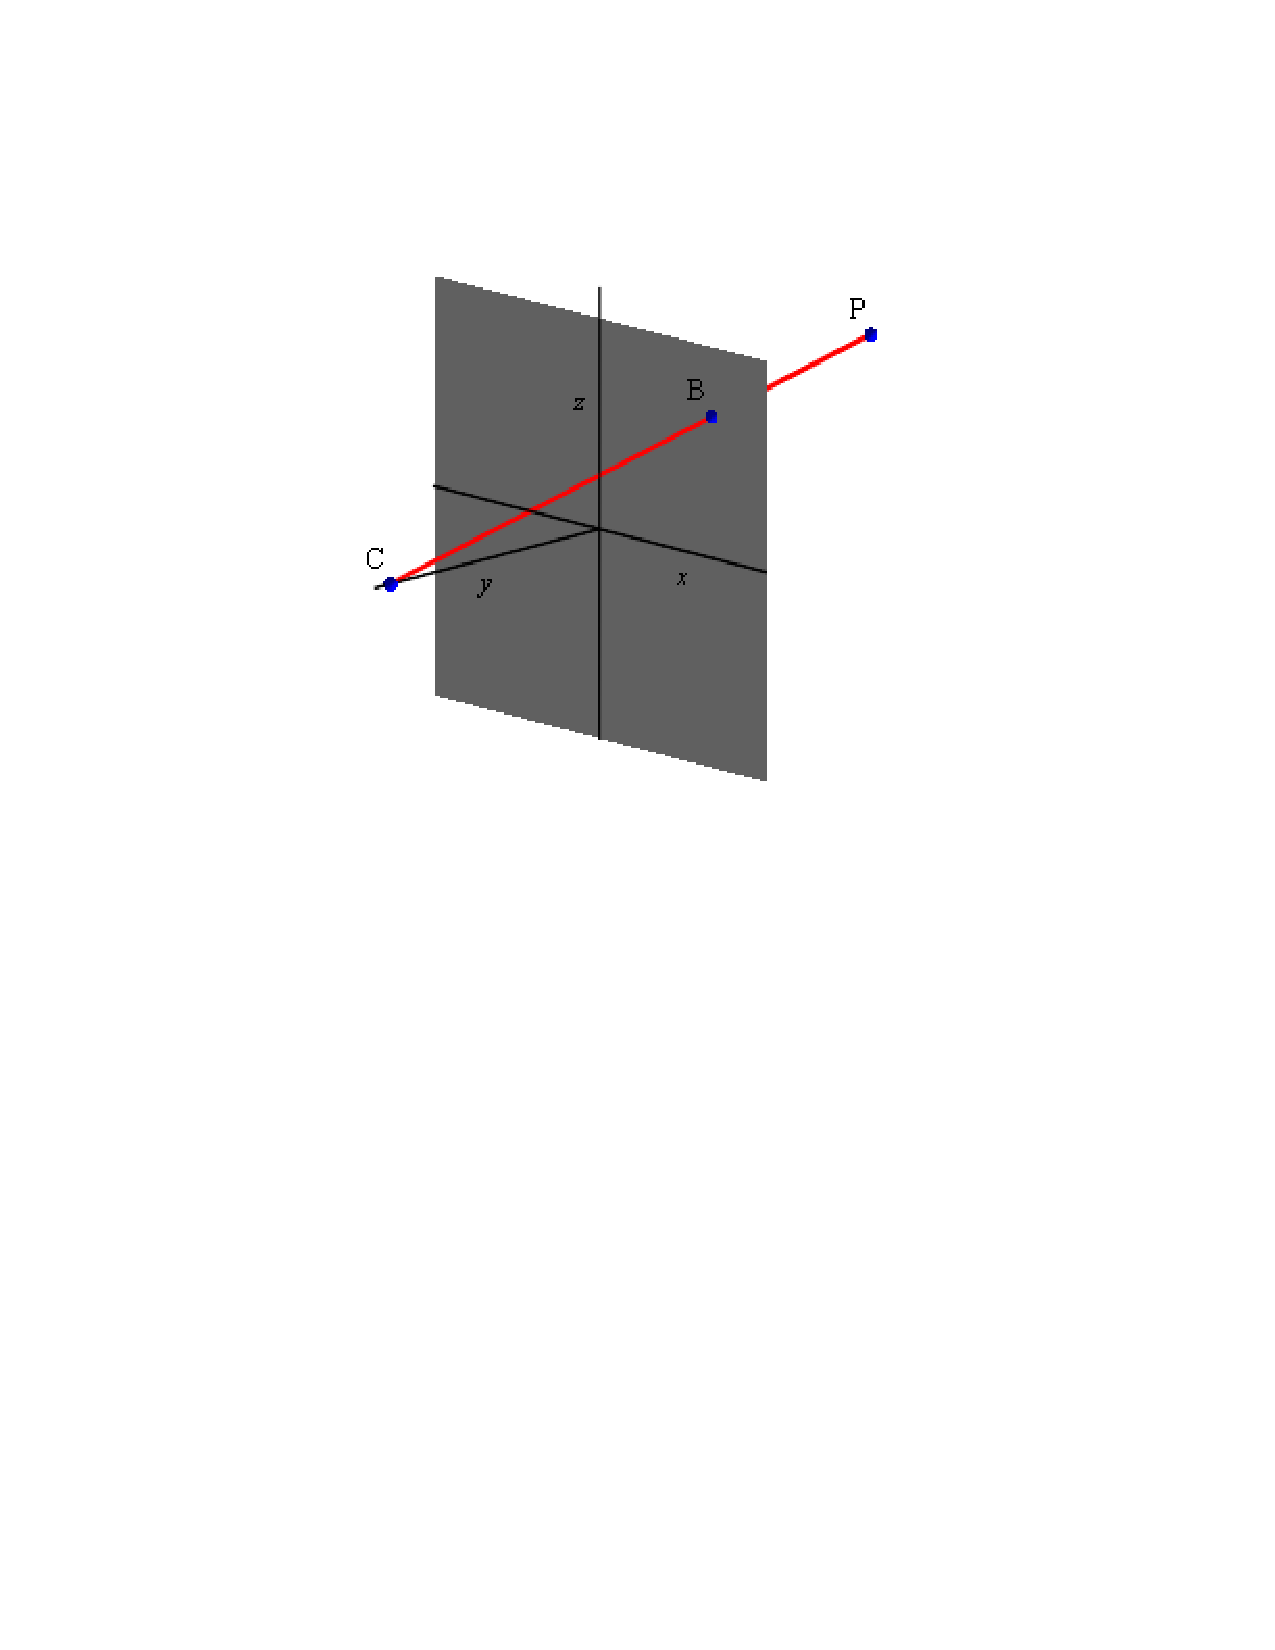
\includegraphics[width=5cm]{perspektiv_projektion}
  \caption{Viser princippet bag perspektiv projektion af et punkt på et billedplan.}
\end{figure}

Som vist på figur \ref{fig:perspektiv_projektion} kan et punkt $P\in \mathbb{R}^3$ projekteres ned på billedplanen $\alpha$ ved at finde skæringspunktet $B$ mellem billedplanen $\alpha$ og en lysstråle $L$, som går fra punktet $P$ mod kameraets position $C$. Gør man nu dette for alle punkter på et objekt i rummet, og tegner skæringspunkterne på billedplanen, dannes et billede af objektet. Udfordringen er så at afgøre hvilken farve punkterne på billedplanen skal have, da dette til dels afhænger af objektets farve, men også hvilket udefrakommende lys der rammer objektet. 

For at løse denne udfordring, benytter vi i dette projekt raytracing, der som beskrevet under afsnit \ref{sec:computergrafik}, bygger på at simulere lysstrålers interaktion med forskellige objekter i rummet. Hvordan dette fungere er beskrevet i næste afsnit, hvor der opstilles en model for en backwards raytracing.

\paragraph{Raytracing}
I modsætning til en perspektiv projektion af et punkt på et plan, er raytracing, hvor man i stedet for punktet i rummet, tager udgangspunkt i de lysstråler der danner billedet. Ved backwards raytracing følger man lysstrålerne baglæns og ser på, hvor stor en lysintensitet, den pågældende lysstråle har efter den har interageret med objekterne i rummet. Ud fra dette farves det tilhørende punkt på billedet, og på den måde kan man rendere et helt billede. På figur \ref{fig:raytracing_skitse} er det vist hvordan man kan konstruere en lysstråle ud fra et bestemt punkt på billedplanen, hvor lysstrålen er beskrevet ved en retningsvektor og et startpunkt.

\begin{figure}[H]
  \label{fig:raytracing_skitse}
  \centering
  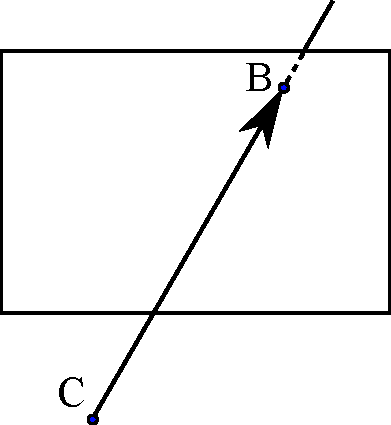
\includegraphics[width=5cm]{drawing}
  \caption{Viser hvordan en der kan opstilles retningsvektor mellem kameraets position $C$ og punktet $P$ på billedplanen, som sammen med startpunktet $C$ beskriver lysstrålen i omvendt retning.}
\end{figure}

Der findes flere forskellige modeller for hvordan lysintensiteten for en lysstråle beregnes. En simpel model, er Phong-modellen, som opdeler lys i forskellige kategorier: ambient, diffuse og specular.

\subsubsection{Konvertering fra farvetemperatur til RGB}
Farvetemperatur, som også er beskrevet nederst i \ref{sec:lys}, er temperaturen af et udsendt lys og måles i kelvin. Denne temperatur kan bruges til at finde ud af, om et lys er varmt eller koldt. 
RGB-værdien er en værdi for en given farves indhold af rød, grøn og blå. Værdien angives normalt ved et tal mellem 0 og 255, altså er 0 128 255 ingen rød, en del grøn og fuld blå, hvilket, blandet sammen, giver en blålig farve.
Der findes ingen direkte og 100\% præcis formel for at ’oversætte’ en kelvintemperaturværdi til en RGB-værdi, derfor har rapporten taget udgangspunkt i en forholdsvis præcis algoritme, som er lavet ud fra 800 målinger, men som stadig ikke er præcis nok til videnskabelig brug.
Måden hvorpå algoritmen er lavet, er ved at tage disse 800 målinger, og lave en funktion ud fra dem. Der er lavet to målinger per 100 kelvin, der starter ved 1000 kelvin og slutter ved 40.000 kelvin. Ved at kigge på funktionen set her: \href{http://www.tannerhelland.com/4435/convert-temperature-rgb-algorithm-code/raw_temperature_vs_rgb_chart/}{http://www.tannerhelland.com/}har Tanner Helland  kunne konkludere  tre ting:


•	Røde værdier under 6600 kelvin er altid 255.


•	Blå værdier under 2000 kelvin er altid 0.


•	Blå værdier over 6500 kelvin er altid 255.


Disse tre, forholdsvis simple, konklusioner har hjulpet med at gøre algoritmen meget kortere og mere simpel. Algoritmen tager et input i kelvin, af typen unsigned int, beregner de tre RBG-værdier hver for sig, og returnerer herefter RGB-værdien, af typen pixel, til sidst. 


\subsubsection*{Opsummering}

[Kort opsummerende beskrivelse af teorierne]